\section{Aufbau und Durchführung}
\subsection{Aufbau}

Die in dem Versuch verwendte Wärmepumpe besteht aus zwei Wasser Reservoiren mit jeh Drei Litern Fassungsvermögen.
Durch diese läuft ein Kupferrohr in welchem sich das Transportgas Dichlordifluormethan befindet.
Der Kompressor pump das Gas mit hohem Druck, welcher durch den Wiederstand des Drosselventils ermöglicht wird, in Reservoir 1 wodurch es sich erhitzt.
In Reservoir 1 verflüssigt es aufgrund des hohen Druckes und des Temperaturabfalls.
Dach dem durchlaufen des Drosselventils fängt das flüssige Gas an wieder zu verdampfen und ist nachdem es Reservoir 2 durchlaufen hat wieder vollständig gasförmig und hat bei dem Phasenwechsel Wärmeenergie aus Reservoir 2 aufgenommen.
Nachdem durchlaufen des 2. Reservoirs wird das gas erneut von dem Kompressor gepumpt und der Kreislauf beginnt von vorn.
Im Fall des Versuchsaufbaus beziehungsweise zur tatsächlichen Technischen Umsetzung werden noch weite Komponenten benötigt wie zu Beispiel ein Reiniger welcher sich vor dem Drosselventil befindet und dafür zuständig ist das verflüssigte Gas von gasförmigen Resten zu befreien,
eine Steuerung welche das Drosselventil steuert sowie Rührer welche den Wärmeaustausch zwischen dem Kupferrohr und dem Wasser beschleunigen.
Außerdem sind im Falle des Versuchsaufbaus noch vor und nach dem Drosselventil Messgeräte für den Druck sowie Thermometer in den beiden Reservoiren angebracht.
\begin{figure}[H]
  \centering
  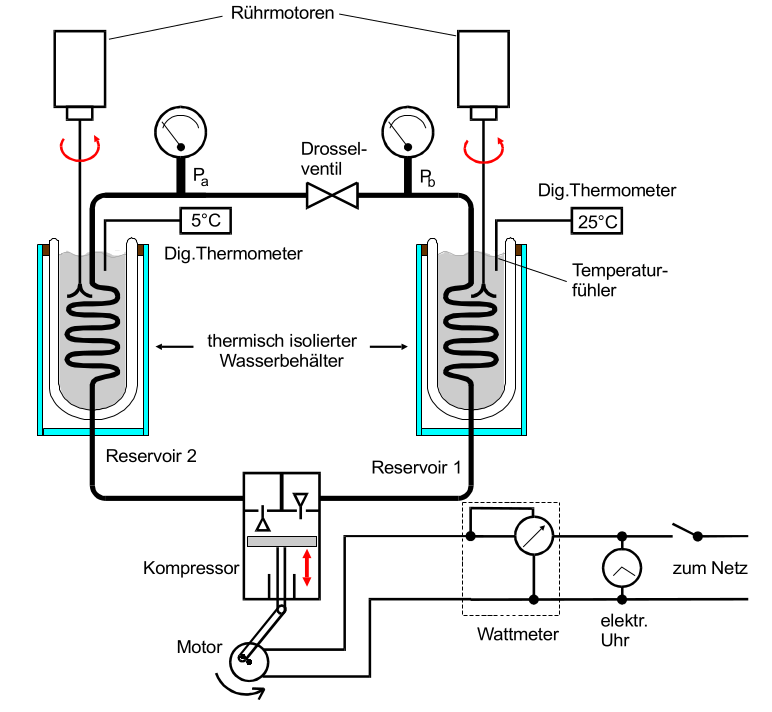
\includegraphics[width=0.6\textwidth]{assets/aufbau.png}
  \caption{Versuchsaufbau}
  \label{fig:aufbau}
\end{figure}
\subsection{Durchführung}
Am Anfang des Experimentes werden die beiden Reservoire mithilfe eines Messkolben mit 3 Litern Wasser befüllt. Nach Einbau der beiden Reservoire
in die Apparatur werden die Rührmotoren und der Kompressor eingeschaltet. Nun werden im Abstand von einer Minute die verschiedenen Drücke und Temperaturen
von Reservoir 2 [$p_a, T_2$] und Reservoir 1 [$p_b, T_1$], sowie die duch den Kompressor eingebrachte Leistung $L$ gemessen und notiert.
Sobald die Temperatur im Reservoir 1 die 0 °C Marke unterschreitet, wird der Kompressor wieder ausgeschaltet.
Bei den Druckmesssungen ist zu beachten, dass diese einen Versatz von $-1 \si{\bar}$ haben, welcher im Folgenden auf alle Druckmesssungen aufaddiert wurde.
